\title{Lecture 19\\Representation of Problems and Their Solutions in a Knowledge Base}

\begin{frame}
	\titlepage
\end{frame}

\begin{frame}{\\Lecture outline}
	\topline
	\justifying
	\setlength{\emergencystretch}{2em}
	Problems and their classification. Information and behavioral problems. Declarative and procedural problem formulations. Action execution plans, protocols, and results. Examples of representing a solution in a knowledge base. Commands and how users work with them in interfaces of next-generation computer systems.
\end{frame}

\begin{frame}{\\The concept of a problem}
	\topline
	\justifying
    \begin{SCn}
    \scnheader{problem}
    \scnidtf{description of a desired state or event in either the knowledge base or the external environment}
    \scnidtf{problem formulation}
    \scnidtf{task to carry out an action}
    \scnidtf{problem statement}
    \scnidtf{problem situation}
    \scnidtf{specification of an action that is complete enough to allow the action to be carried out}
    \end{SCn}
\end{frame}

\begin{frame}{\\The concept of a problem}
	\topline
	\justifying
    \textbf{\textit{A problem}} is specified by a relation between a description of the initial situation and a description of the goal situations.\\

    \bigskip

    Each \textbf{\textit{problem}} specifies an action that has already been completed, is currently in progress, is planned or required, or may be carried out (without being required).
\end{frame}

\begin{frame}{\\Classification of problems}
	\topline
	\justifying

    Problems can be classified by didactic or logical criteria within each subject domain (problems involving triangles, systems of equations, etc.)\\
    \bigskip
    Each \textit{problem} can include:
    \begin{textitemize}
        \item the fact that the \textit{action} belongs to a specific class of \textit{actions}, including its lifecycle state (initiated, in progress, etc.);
        \item a description of the \textit{goal*} (\textit{result*}) of the \textit{action}, if it is known precisely;
        \item identification of the action's \textit{requester*};
        \item identification of the \textit{performer* of the action};
    \end{textitemize}
\end{frame}

\begin{frame}{\\Classification of problems}
	\topline
	\justifying

    \bigskip
    Each \textit{problem} can include:
    \begin{textitemize}
        \item identification of the \textit{argument(s) of the action\scnrolesign};
        \item identification of a tool or intermediary for the \textit{action};
        \item a description of the \textit{action decomposition*};
        \item specification of the \textit{sequence of actions*} within the \textit{action decomposition*}, thereby defining a procedural plan for solving the problem;
        \item specification of the scope of the \textit{action};
        \item specification of the initiation condition of the \textit{action};
        \item the start and end times of the \textit{action}, including planned and actual times, and its expected and/or actual duration.
    \end{textitemize}
\end{frame}

\begin{frame}{\\Classification of problems}
    \topline
	\justifying

    \bigskip

    Context can further specify some problems by providing additional information about the entities in the \textit{problem} formulation, such as what is given or already known about them.\\
    \bigskip

    A \textit{problem} can also include any additional information about the action, for example:
    \begin{textitemize}
        \item the resources and means expected to be used in solving the problem;
        \item limits on the scope of the \textit{action};
        \item limits on the knowledge that may be used to solve the problem.
    \end{textitemize}
\end{frame}

\begin{frame}{\\Information and behavioral problems}
	\topline
	\justifying

    As with the actions a system carries out, problems can be classified as \textit{information problems} or \textit{behavioral problems}.
    Problems can also be distinguished by how they are formulated, as \textit{declarative problem formulations} or \textit{procedural problem formulations}. A formulation may combine both approaches.
\end{frame}

\begin{frame}{Declarative and procedural formulations}
	\topline
	\justifying

    \begin{SCn}
    \scnheader{problem}
    \scnsuperset{question}
    \scnsuperset{command}
    \scnsubset{knowledge}
    \scnsuperset{initiated problem}
    \scnsuperset{declarative problem formulation}
    \scnsuperset{procedural problem formulation}
    \scnsuperset{declarative-procedural problem formulation}
    \scnsuperset{problem solved in the memory of a cybernetic system}
    \end{SCn}
\end{frame}

\begin{frame}{Declarative and procedural formulations}
	\topline
	\justifying

    \textbf{\textit{declarative problem formulation}} describes the initial situation that serves as the condition for carrying out the action and the goal situation that results from it. The goal situation describes the state the planned action must achieve.
\end{frame}

\begin{frame}{Declarative and procedural formulations}
	\topline
	\justifying
	\small
	\par\vspace{8mm}
     A \textbf{\textit{procedural problem formulation}} explicitly specifies characteristics of the action, for example:
    \begin{textitemize}
    \item the subject or subjects that carry out the action;
    \item the objects on which the action is performed, i.e., its arguments;
    \item the tools used to carry out the action;
    \item the times and any additional conditions for starting and completing the action;
    \item the class membership of each \textit{action}.
    \end{textitemize}

	The formulation leaves the expected result of the corresponding action unspecified.

\end{frame}

\begin{frame}{Declarative and procedural formulations}
	\topline
	\justifying
	\vspace{10mm}

    If necessary, a \textit{procedural problem formulation} can be reduced to a \textit{declarative problem formulation} by translating it according to a rule, for example, by defining the class of the action in terms of a more general class.

    \bigskip

    A declarative-procedural problem formulation includes both declarative (goal-oriented) and procedural aspects. An initiated problem is a problem formulation that is to be carried out.

\end{frame}

\begin{frame}{\\Specific types of problems}
    \topline
	\justifying
    \begin{SCn}
    \scnheader{question}
    \scnsubset{problem solved in the memory of a cybernetic system}
    \scnidtf{non-procedural formulation of a problem of finding knowledge (in the current state of the knowledge base) or generating knowledge that satisfies given requirements}
    \scnidtf{problem aimed at satisfying the information needs of a requester}
    \scnheader{command}
    \scnidtf{initiated problem}
    \scnidtf{specification of an initiated action}
    \end{SCn}
\end{frame}

\begin{frame}{\\Action execution plan}
	\topline
	\justifying
    \scnheader{action execution plan}
    \scnidtf{procedural program}
    \scnidtf{specification of the decomposition of any action that belongs to a given class of actions}
\end{frame}

\begin{frame}{\\Action execution protocol}
	\topline
	\justifying
    \scnheader{action execution protocol}
    \scnidtf{description of how the action was actually carried out, including the sequence of corresponding situations and events}
    \scnidtf{decomposition of a completed action into its sequentially and concurrently executed
subactions}

\end{frame}

\begin{frame}{\\Action execution result}
	\topline
	\justifying

    \bigskip

    Result is the relation linking the sc-element that denotes an action to the sc-construct describing its outcome, i.e., the goal to be achieved by carrying out the action.\\
    A result can be specified by an atomic proposition or a non-atomic one, such as a conjunctive, disjunctive, or exclusive-disjunctive proposition.\\

    \bigskip

    If successful execution changes a construct in sc-memory and that change must be recorded in the knowledge base history or shown in the problem-solving protocol, a tuple of the result* relation is generated. It links the problem to the sc-construct describing the change.
\end{frame}

\begin{frame}{\\The concept of a command}
	\topline
	\justifying
	\vspace{10mm}

    \scnheader{command}
    \scnidtf{initiated problem}
    \scnidtf{specification of an initiated action}

   \bigskip

   In Russian, the identifier of an instance of a particular command class begins with a capital letter. It either uses a perfective infinitive to describe what the command's action should produce or uses a question to specify the requested information.

   \bigskip

   Examples:
   \begin{textitemize}
        \item "What is a triangle?"
        \item "Generate a new instance of the class triangle"
   \end{textitemize}

\end{frame}

\begin{frame}{\\Example of a problem statement}
	\topline
	\justifying
	\vspace{10mm}
	\begin{SCn}
		\begin{figure}[H]
			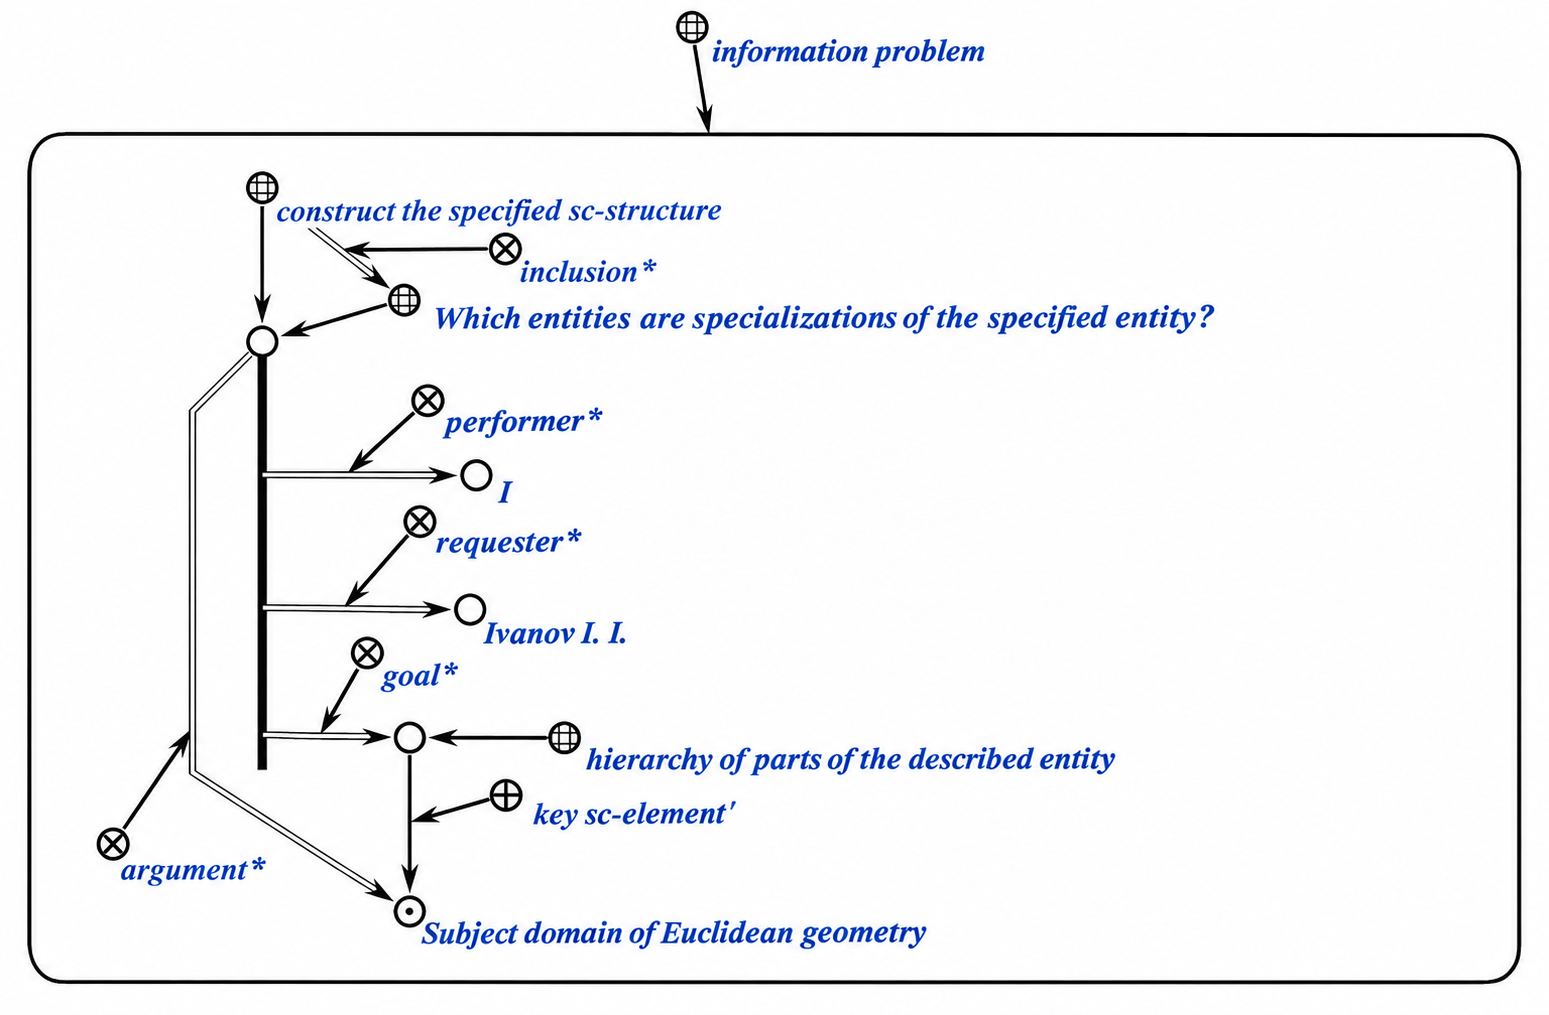
\includegraphics[width=\linewidth,height=0.68\textheight,keepaspectratio]{figures/sd_problems/entities_en.png}
		\end{figure}
	\end{SCn}
\end{frame}

\begin{frame}{\\Example of a problem statement}
	\topline
	\justifying
	\vspace{10mm}
	\begin{SCn}
		\begin{figure}[H]
			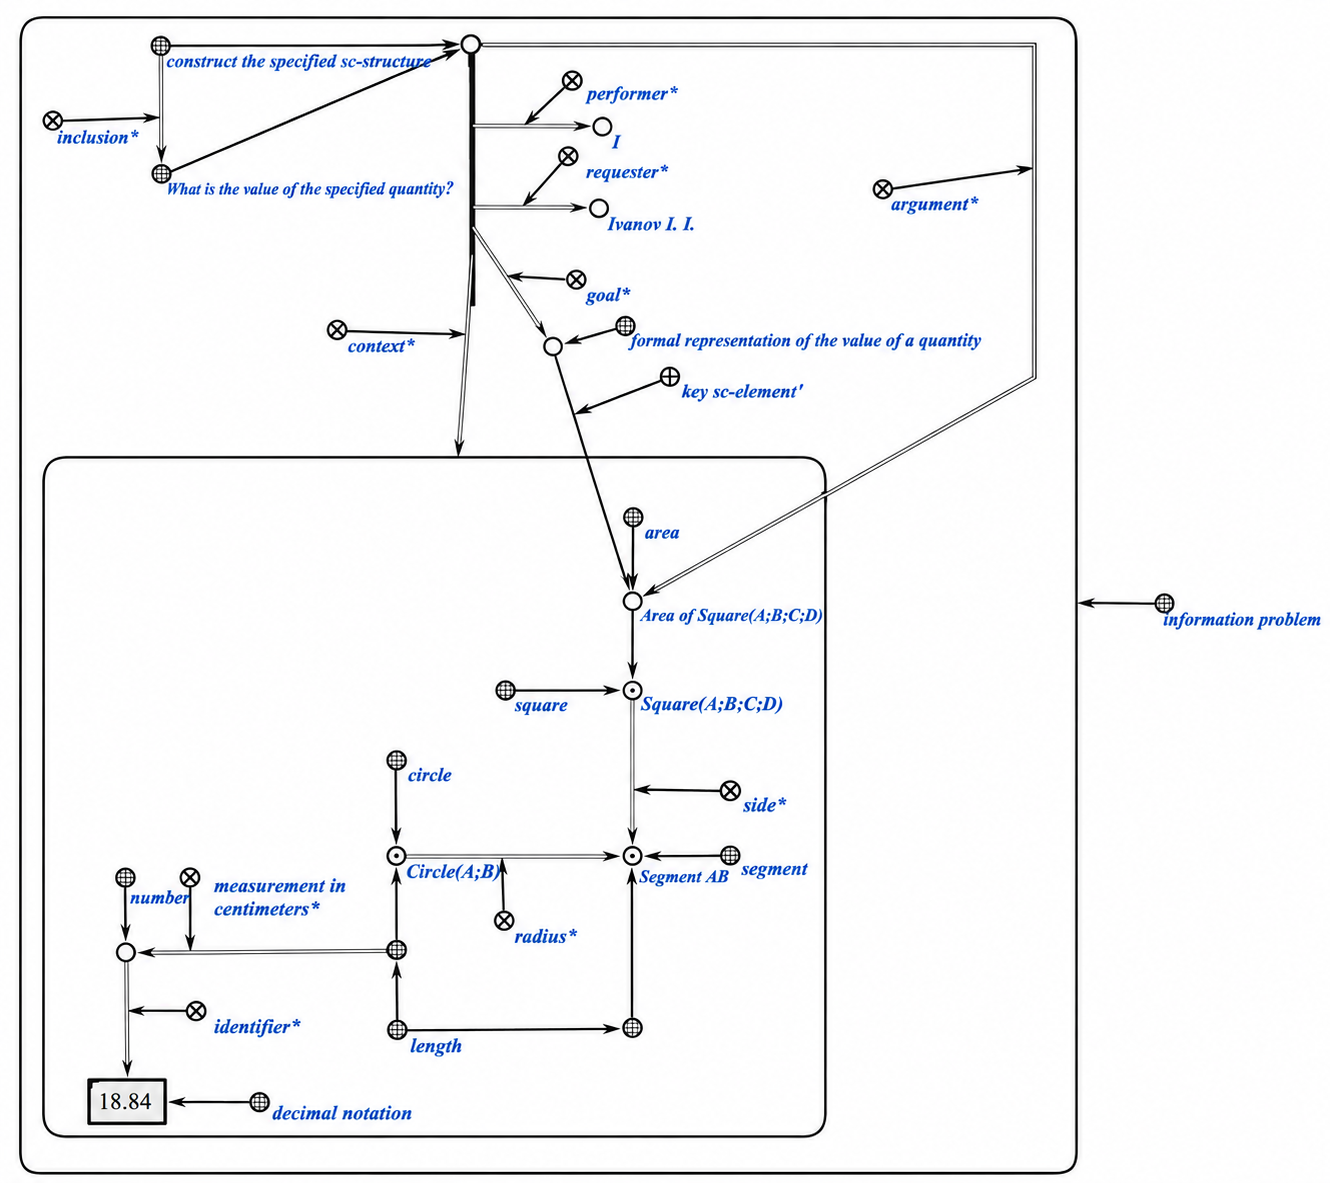
\includegraphics[width=\linewidth,height=0.71\textheight,keepaspectratio]{figures/sd_problems/value_en.png}
		\end{figure}
	\end{SCn}
\end{frame}


\begin{frame}{\\Example of a problem solution}
	\topline
	\justifying
	\vspace{10mm}
	\begin{SCn}
		\begin{figure}[H]
			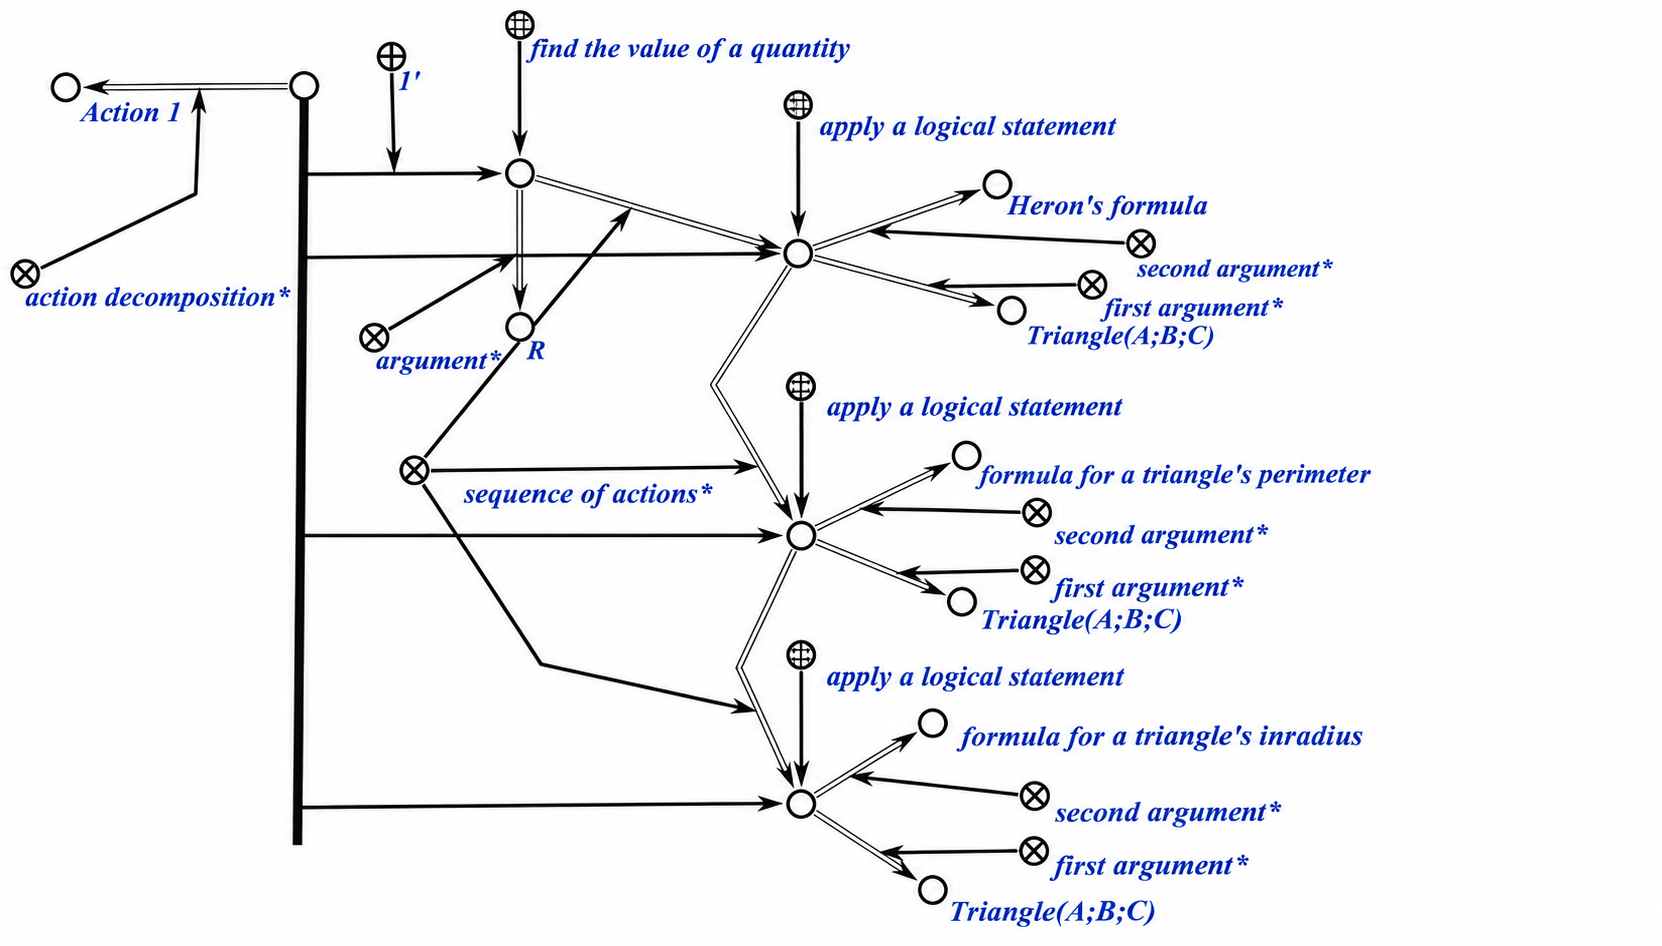
\includegraphics[width=\linewidth,height=0.68\textheight,keepaspectratio]{figures/sd_problems/solution_en.png}
		\end{figure}
	\end{SCn}
\end{frame}
